\documentclass[12pt,UTF8]{ctexart}
\usepackage{titling,setspace}
\usepackage{enumerate,enumitem}
\usepackage{amsmath,amssymb,amsfonts}
\usepackage{listings}
\usepackage{comment}
\usepackage{float}
\usepackage{graphicx}
\usepackage{multicol,multirow}
\usepackage[unicode=true,%本行非常重要 支持中文目录hyperref CJKbookmarks对二级目录没用
	colorlinks,
	linkcolor=black,
	anchorcolor=black,
	citecolor=black,
	CJKbookmarks=false]{hyperref}
\usepackage{xcolor}
\usepackage{geometry}
\geometry{top=25mm,bottom=25mm,left=25mm,right=25mm}
\pagestyle{plain}%删除页眉
\CTEXsetup[format={\large\bfseries}]{section}
\renewcommand\maketitlehooka{\null\mbox{}\vfill} % 标题页
\renewcommand\maketitlehookd{\vfill\null}

\lstset{language=c++,basicstyle=\tiny,escapechar=`,showstringspaces=false}
\setlength{\droptitle}{-100pt}%减少标题与页眉距离

\setenumerate[1]{itemsep=0pt,partopsep=0pt,parsep=\parskip,topsep=5pt}
\setitemize[1]{itemsep=0pt,partopsep=0pt,parsep=\parskip,topsep=5pt}

\title{{\Huge Project 4\\校园导游}}

\vspace{100pt}
\author{\vspace{200pt}\quad\\
计科一班 17341009 曾天宇\\
计科一班 17341015 陈鸿峥\\
计科二班 17341059 黄杨峻}
\date{}

\begin{document}
\begin{spacing}{1.4}

\clearpage\maketitle
\thispagestyle{empty}

\newpage
\setcounter{page}{1}
\section{题目要求}
\begin{enumerate}
	\item 从中山大学东校区的平面图中选取有代表性景点(20-30个),抽象成一个无向带权图。以图中顶点表示校内各景点,存放景点名称、代号、简介等信息;以边表示路径,存放路径长度等信息。
	\item 为来访客人提供图中任意景点相关信息的查询。
	\item 为来访客人提供图中任意景点的问路查询,即查询任意两个景点之间一条最短的简单路径。
	\item 区分汽车线路与步行线路。
\end{enumerate}
\begin{figure}[H]
\centering
\includegraphics[width=0.6\linewidth]{fig/EastCampus.jpg}
\end{figure}

\section{数据结构与算法}
由于这次的题目较为简单,若单纯做一个算法实现那没什么意思,故我们想挑战一下自己:将其做成项目,并实现全平台导览,包括PC端(网页版)、微信小程序(Android)及iOS设备。详情见下面的描述。

\subsection{PC端(网页版)实现}
\subsubsection{使用语言}
html、javascript、css

\subsubsection{设计思想}
设计一个PC端(网页)实现校园导览。
\par 调用百度地图的API求得两点之间的路径长度,存入矩阵,用Dijkstra算法求得两点的最短路径,在地图上将路径、路径描述、相关地点简介、途径点进行显示。
网页作品已上传至服务器\url{http://193.112.60.186:81/CampusMap.html},保留期限为本学期。

\subsubsection{数据结构}
采用邻接矩阵存储各顶点间的距离。
\par 定义了地图的\verb'container',定义了文本框\verb'ui-box',按钮\verb'button'等类的结构。

\subsubsection{算法过程}
\begin{enumerate}
	\item 在网页上抓取用户输入的起点和终点,调用查询\verb'search()'函数
	\item 在预定义的数组中得到起点和终点的经纬度坐标,调用百度API中步行或驾车的\verb'search()'函数展示路径
\begin{figure}[H]
\centering
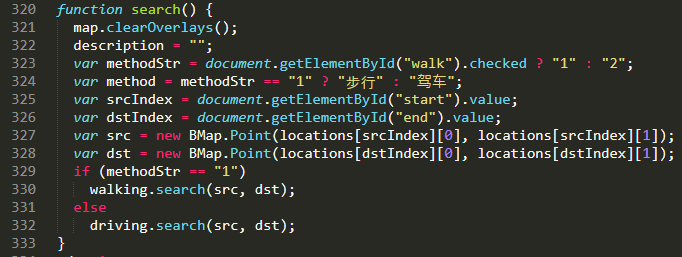
\includegraphics[width=0.6\linewidth]{fig/search.PNG}
\end{figure}
	\item 另一方面,调用\verb'getAdjPoints'函数,用Dijkstra算法(见下图)求得要连接这两点最短路径的中间点(由于已预定义了两点之间的相对距离,存在矩阵内,故可以求SSSP,而无需在运行时再重新估算距离),在地图上显示出来,并在侧边文本框输出景点简介
\begin{figure}[H]
\centering
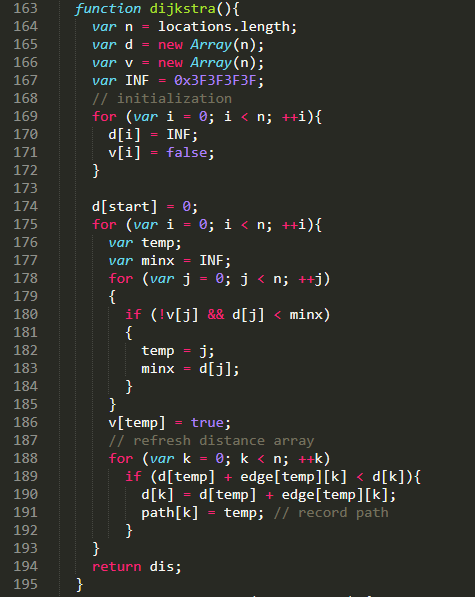
\includegraphics[width=0.5\linewidth]{fig/dijkstra.PNG}
\end{figure}
	\item 搜索结束后在地图上标注路径、起点、终点、途径点,并在侧边文本框输出全程距离和具体路径实施规划
\end{enumerate}

\subsubsection{测试截图}
\begin{figure}[H]
\centering
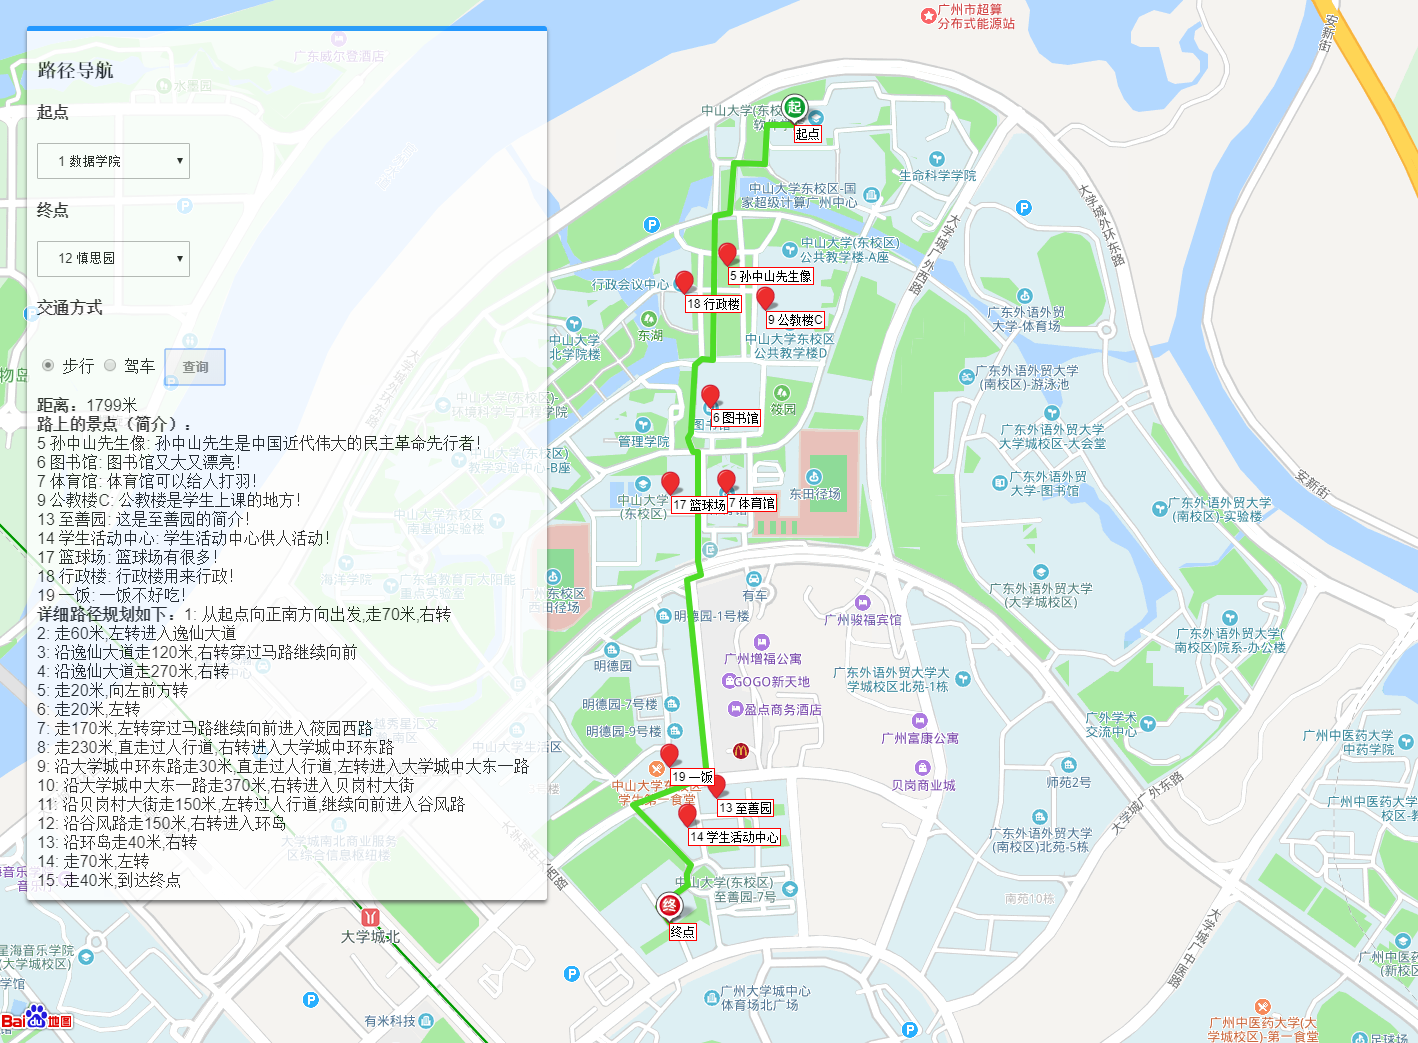
\includegraphics[width=0.8\linewidth]{fig/web1.PNG}
\end{figure}
\begin{figure}[H]
\centering
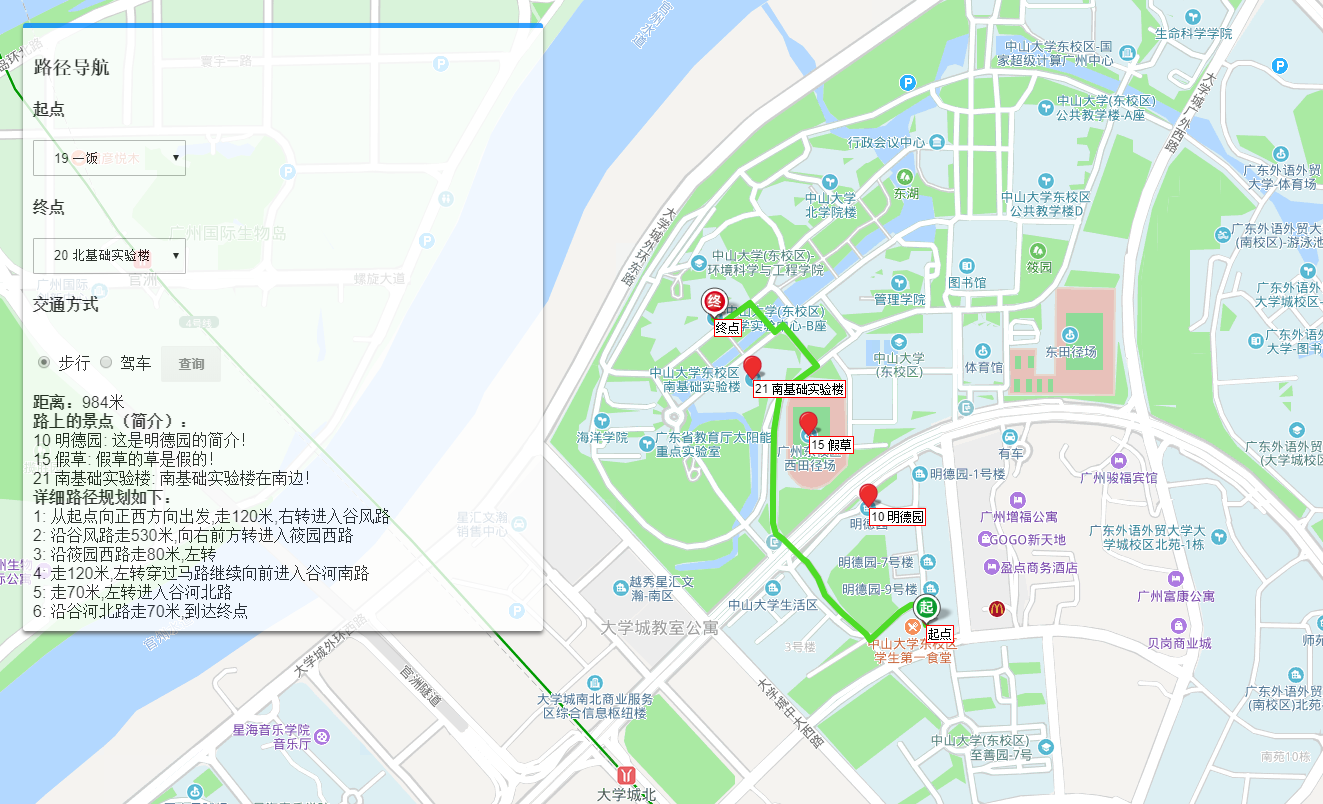
\includegraphics[width=0.8\linewidth]{fig/web2.PNG}
\end{figure}
由于驾车路线涉及到的问题比较多,还在开发,故这里没有给出相应截图。


\subsection{微信小程序实现}
\subsubsection{使用语言}
wxml、wxss、js、json

\subsubsection{设计思想}
设计一个微信小程序实现题目要求,使得手机移动端(iOS和Android)可用。调用腾讯地图的API,实现从点到点的路径规划,并显示途径的景点。

\subsubsection{数据结构}
定义了Placelist类,存储所有景点的信息(包括经纬度、地点名称等)
\begin{lstlisting}
Placelist({
	id: ,
	latitude: ,
	longitude: , 
	placeName: '___'
})
\end{lstlisting}
定义了Markers类,用于显示地图上的景点气泡,图标根据景点类型而决定(起点、终点、经过点、其他点)
\begin{lstlisting}
Markers({
	Id: ,
	Latitude: ,
	Longitude: ,
	iconPath:'___',
	Height: ,
	Width: ,
	Callout{
		Content:'___',
		Display:'___'
	}
})
\end{lstlisting}
Polyline:用于存储请求API返回的路径\verb'Polyline[(longitude,latitude)]'

\subsubsection{算法过程}
\begin{enumerate}
	\item 寻路:首先定义景点之间的距离为一个邻接矩阵(相当于一个导游图),然后通过在线Dijkstra算法求最短路径(抽象),最后通过API逐段请求路径中每两个景点的真实路径,将其push到polyline这个list里面,拼接成完整的路径
	\item 中间点:由于景点不一定在路上,所以采用标准化欧氏距离$<0.0000003$来衡量中间点。
\end{enumerate}

\subsubsection{测试截图}
\begin{figure}[H]
\centering
\begin{tabular}{cc}
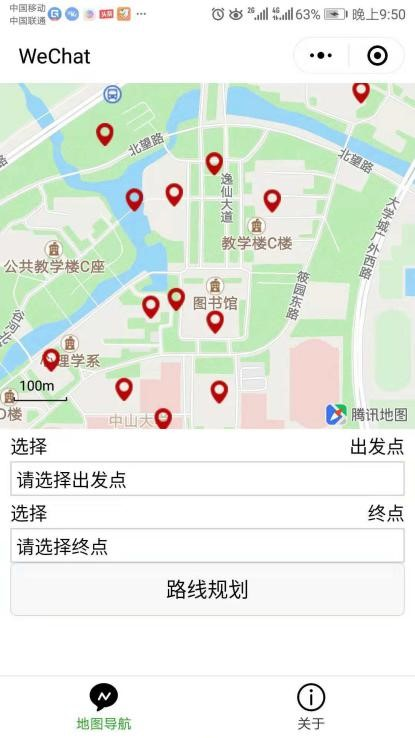
\includegraphics[width=0.3\linewidth]{fig/wechat1.jpg}&
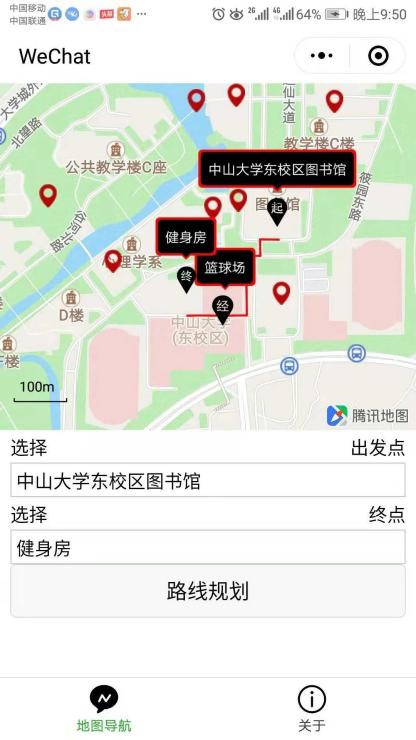
\includegraphics[width=0.3\linewidth]{fig/wechat2.jpg}
\end{tabular}
\end{figure}
\begin{figure}[H]
\centering
\begin{tabular}{cc}
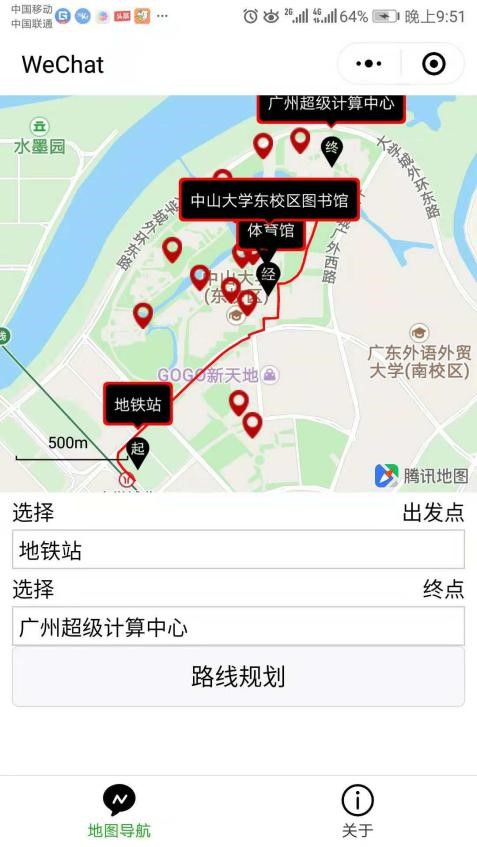
\includegraphics[width=0.3\linewidth]{fig/wechat3.jpg}&
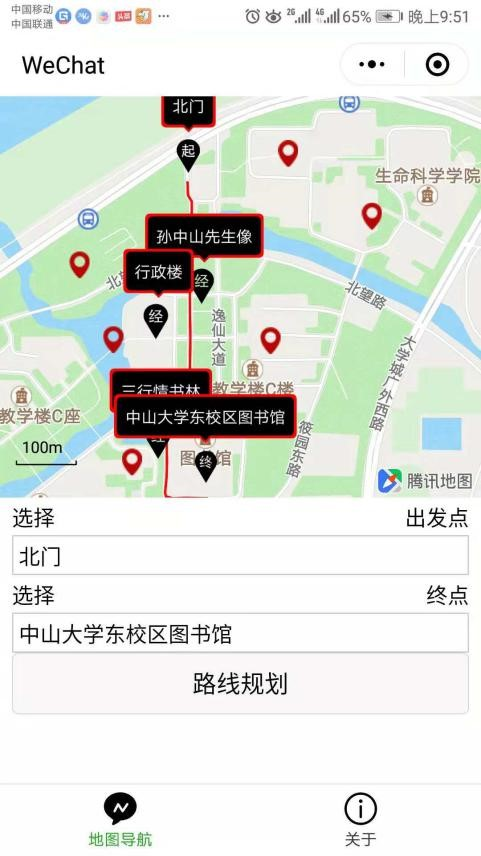
\includegraphics[width=0.3\linewidth]{fig/wechat4.jpg}
\end{tabular}
\end{figure}

\subsubsection{不足之处}
\begin{enumerate}
	\item 响应速度不够,没有设置加载中的圈圈以减少用户焦虑
	\item Markers的气泡太丑,而且透明度不足
	\item 无法支持实时导航(因为没权限)
\end{enumerate}


\subsection{iOS平台实现}
\subsubsection{使用语言}
Swift、Objective-C

\subsubsection{设计思想}
设计一个iOS APP实现题目要求,能够支持有序浏览和无序浏览,支持线路指示输出,支持多种交通方式,支持多地图,支持多数据集。

\subsubsection{数据结构}
定义了Swift类:Scenery Point储存景点信息,数据从csv文件Places.csv中读取:
\begin{figure}[H]
\centering
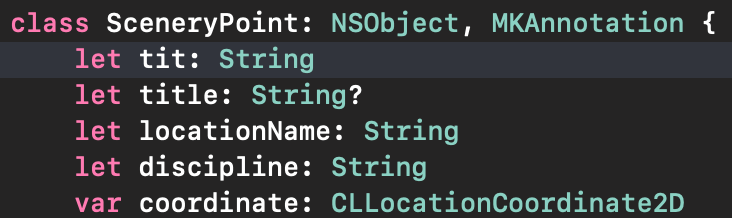
\includegraphics[width=0.5\linewidth]{fig/scenery_point.png}
\end{figure}
定义了Matrix类处理邻接矩阵:
\begin{figure}[H]
\centering
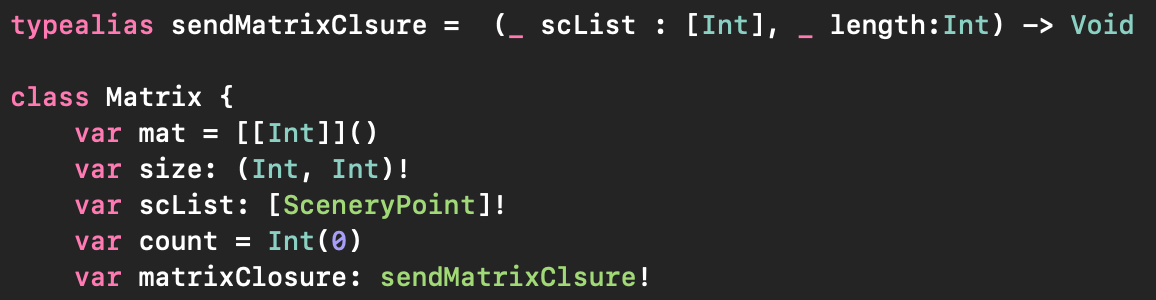
\includegraphics[width=0.5\linewidth]{fig/matrix.png}
\end{figure}
定义了DataListTableCellTableViewCell作为数据显示单元:
\begin{figure}[H]
\centering
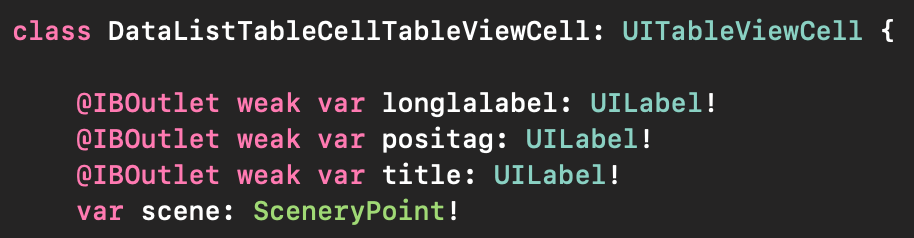
\includegraphics[width=0.5\linewidth]{fig/datalisttable.png}
\end{figure}
定义了 MapClassify 作为数据实时请求处理单元:
\begin{figure}[H]
\centering
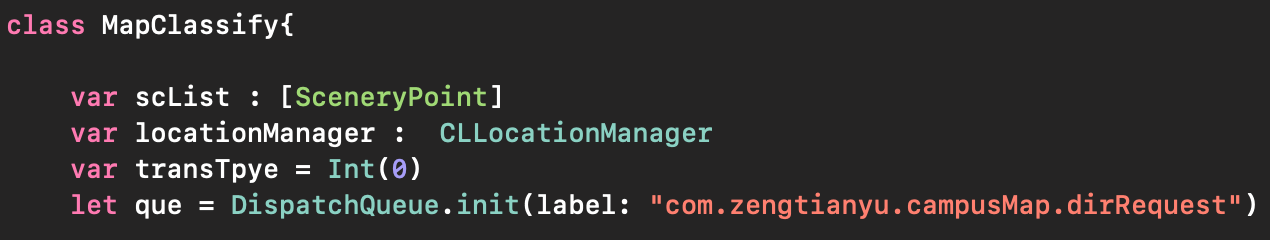
\includegraphics[width=0.5\linewidth]{fig/mapclassify.png}
\end{figure}

\subsubsection{算法过程}
\begin{enumerate}
	\item 有序浏览
有序浏览采用分段请求路径的方式即可实现。通过MKMapView请求得到点对点之间的最小路径,并且显示在MapView上。
	\item 无序浏览
由于是用户先确定浏览点,故无序浏览采用TSP问题的贪心算法。请求点到点之间的有向最小路径,处理邻接矩阵获取最小回路,并将路线显示在MapView上面。
\begin{figure}[H]
\centering
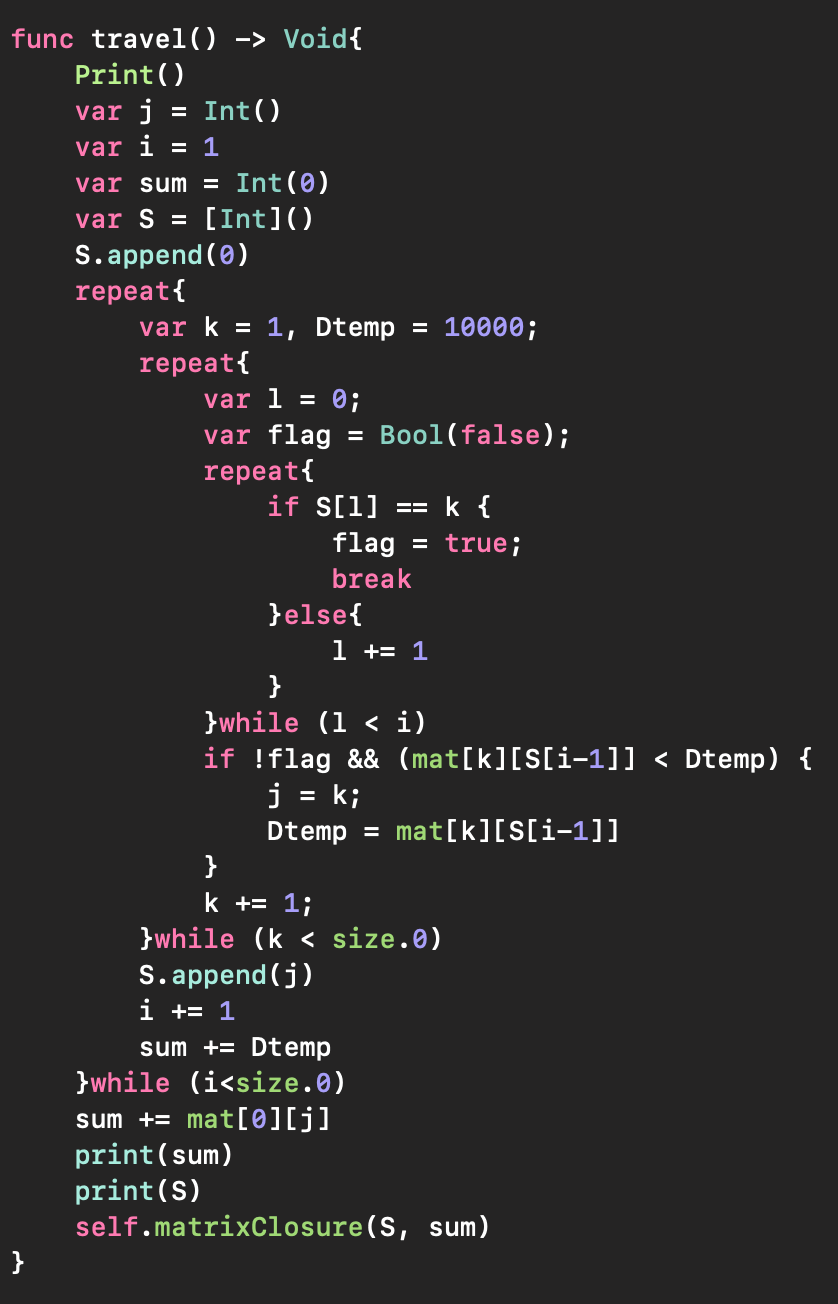
\includegraphics[width=0.4\linewidth]{fig/tsp.png}
\end{figure}
	\item 多线程并发请求处理
MapView中的MKDirection.Request 是一个用于请求路径的类,我们由于需要快速获取路径,所以采用了多线程请求的方式,但是短时多次请求会导致服务器认为这是一个Spam程序,因此做了一定的随机访问处理进行消除。
	\item 串行并行数据冒险消除
由于数据是并行请求的,因此回到串行处理是要使用对应的优化算法和控制方式。iOS提供了DispatchQueue以消除部分数据冒险,我在此基础上进行了改进,添加了串行验证的方式,进一步防止数据冒险。
	\item 显示优化算法
判断用户显示环境,切换对应的地图
	\item 函数闭包返回
\end{enumerate}

\subsubsection{实现功能}
\begin{multicols}{2}
\begin{enumerate}
	\item 2D地图实时显示
	\item 3D地图实时显示
	\item 用户地理位置显示
	\item 用户POI请求
	\item 有序浏览模式
	\item 无序浏览模式
	\item 用户兴趣点显示
	\item 步行浏览模式
	\item 驾车浏览模式
	\item 简单地图显示
	\item 卫星地图显示
	\item 用户地理位置检索
	\item 路线导航与指示
\end{enumerate}
\end{multicols}

\subsubsection{测试截图}
\begin{figure}[H]
\centering
\begin{tabular}{cc}
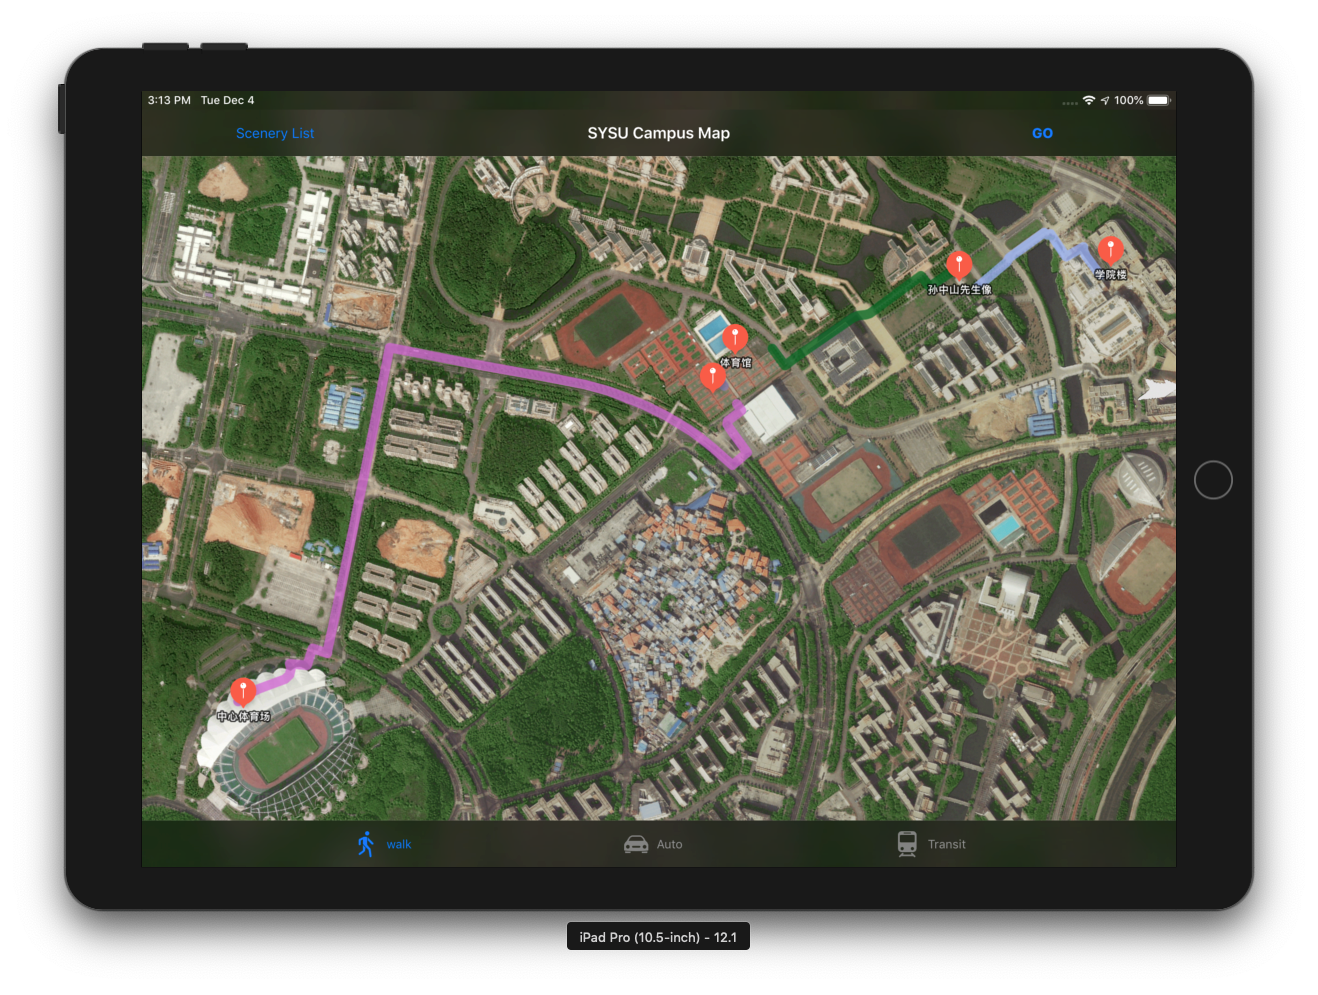
\includegraphics[width=0.7\linewidth]{fig/ios1.png}&
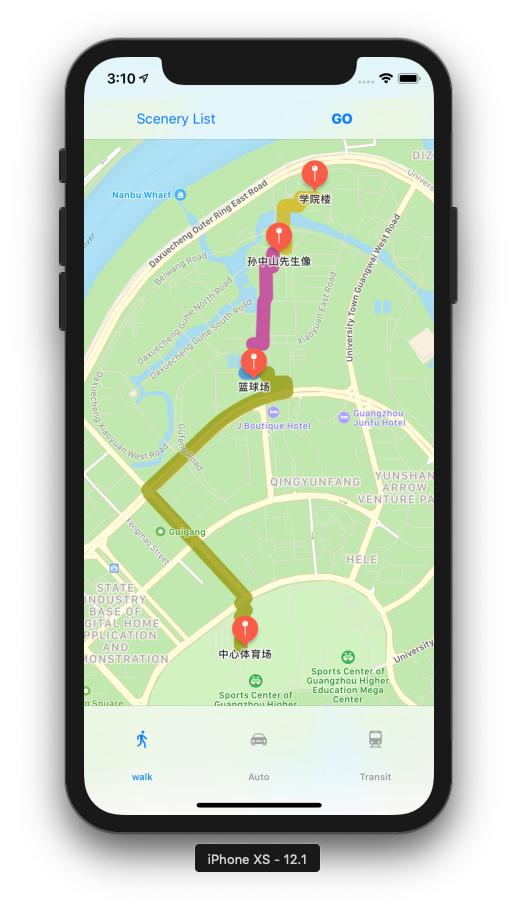
\includegraphics[width=0.3\linewidth]{fig/ios2.png}
\end{tabular}
\end{figure}

\subsubsection{可扩展性}
现在这个软件不仅能够在iOS平台使用,只需要修改40行代码就能够在Mac OS X平台上面运行,真正做到了全平台开发。

\section{分工、贡献与自我评分}
\begin{table}[H]
	\centering
	\begin{tabular}{|c|c|c|c|}
		\hline
		& 分工 & 贡献度 & 自我评分\\
		\hline
		曾天宇 &  完成iOS平台开发,报告撰写 & 0.33 & 10/10\\
		陈鸿峥 &  完成网页端平台开发,报告撰写 & 0.33 & 10/10\\
		黄杨峻 &  完成微信小程序平台开发,报告撰写 & 0.33 & 10/10\\
		\hline
	\end{tabular}
\end{table}

\section{项目总结}
% (收获、体会,若实验课上未完成调试,要认真找出错误并分析原因等。)
本次项目是数据结构课的最后一次项目,虽然最短路径算法实现起来比较简单,但我们想做一些更具有挑战性的事情,所以就想到把项目做大,做成一个全平台可用的应用。总体来说,这次项目汲取了之前几次项目的经验,大家各自用不同语言不同平台开发,最后再整合再一起,有一个完整的效果,还是比较好的。希望我们这种迎难而上的精神以后可以继续保持。

\end{spacing}

%\section{程序清单}
%\subsection{主函数}
%\begin{lstlisting}
%	
%\end{lstlisting}

\end{document}